\documentclass{acm_proc_article-sp}
\usepackage[utf8]{inputenc}

\begin{document}
\title{A Taxonomy of Attacks and Defenses on E-passports}
\subtitle{[State of art]}

\numberofauthors{2} 
\author{
\alignauthor
Aquiles Ricardo TORRES ALVAREZ%\titlenote{Electrical student at Universidad del Norte - Colombia. Double major student of Telecommunication at Ensimag - France}\\
       \affaddr{Grenoble INP - ENSIMAG}\\
       \affaddr{Grenoble, Francia}\\
       \email{torresaa@}
% 2nd. author
\alignauthor
Jorge Luis GULFO MONSALVE%\titlenote{Electrical student at Universidad del Norte - Colombia. Double major student of Telecommunication at Ensimag - France}\\
       \affaddr{Grenoble INP - ENSIMAG}\\
       \affaddr{Grenoble Francia}\\
       \email{gulfomoj@}
}

\maketitle
\begin{abstract}

\end{abstract}

\terms{Theory}

\keywords{passport, MRT, RFID, ICAO, eavesdropping, BAC, attack, cryptography}

\section{Introduction}
The use e-passport or \emph{Machine Readable Travel Document} (\textbf{MRTD}) to speed up the immigration process is growing fast. The promise of eliminate fraud by adding cryptographic protection to traditional passport on a \emph{\textbf{RFID}} chip is the main reason.
The control in borders has been always a defiance for countries because of the compromise of national security therefore the life of millions of people. The \emph{RFID }technology bring up its advantages to help with this problem by carrying the paper readable information and biometrical data in a wireless accessible ship. Additionally, this data is protected by an authentication process to check the truthfulness of passport. Fast, safe and reliable, by far, the best decision. 

Now we know that only “fast” is really true because some attackers have proved that e-passports are not secure and reliable at all as they were originally made for. The \emph{RFID} technology could be the correct once but the regulations of the \emph{International Civil Aviation Organization }(\textbf{ICAO}) for this smart cards have forgot some details. This regulations holes has been used by attackers to find security weaknesses on e-passports.

The remainder of this paper is organized to explain some technical concepts in Section \ref{sec:sec2} and some documented weaknesses of e-passports on Section \ref{sec:sec3}. At Section \ref{sec:sec4} we present our conclusions and some recommendations for the next generations of \emph{MRTD}. 

\section{Technical Background}
\label{sec:sec2}

\subsection{RFID}
The way the E-passport works is by communicating with a RF reader which emits a wave that feeds 
the contactless chip located at the passport which is a Radio Frequency ID or tag. Once he is feeded the exchange of information begins but 
without protection any other RF reader can performs eavesdropping or clone the passport. So, knowing those possibles security issues and privacy threats attached to
the data exchanged between the e-passport and the reader, the \textbf{ICAO} 
(\textit{International Civil Aviation Organization}) has 
established a set of protocols such as \textit{Passive Authentication} (PA), \textit{Basic Access Control} (BAC), 
\textit{Active Authentication} (AA) and \textit{Extended Access Control} (EAC) for encrypting the data.

As mentioned at \cite{NM12} the first protocol to treat was \textit{PA}, which signs the passport with 
a public key of the issuing country in order to prove the integrity and authenticity of the data.

\subsection{BAC Protocol}
As mentioned at \cite{CLPS07}, \textit{BAC} which is a protocol that prevents skimming by encrypting 
the data with two symmetric keys (KE and KM) that are derived from the passport's  
\textit{MRZ} (Machine Readable Zone) (birthdate, the passport’s expiry date and the alphanumeric 
passport number). Once the reader is authenticated all the passport information of the holder are contemplated.

\begin{figure}
  \centering
  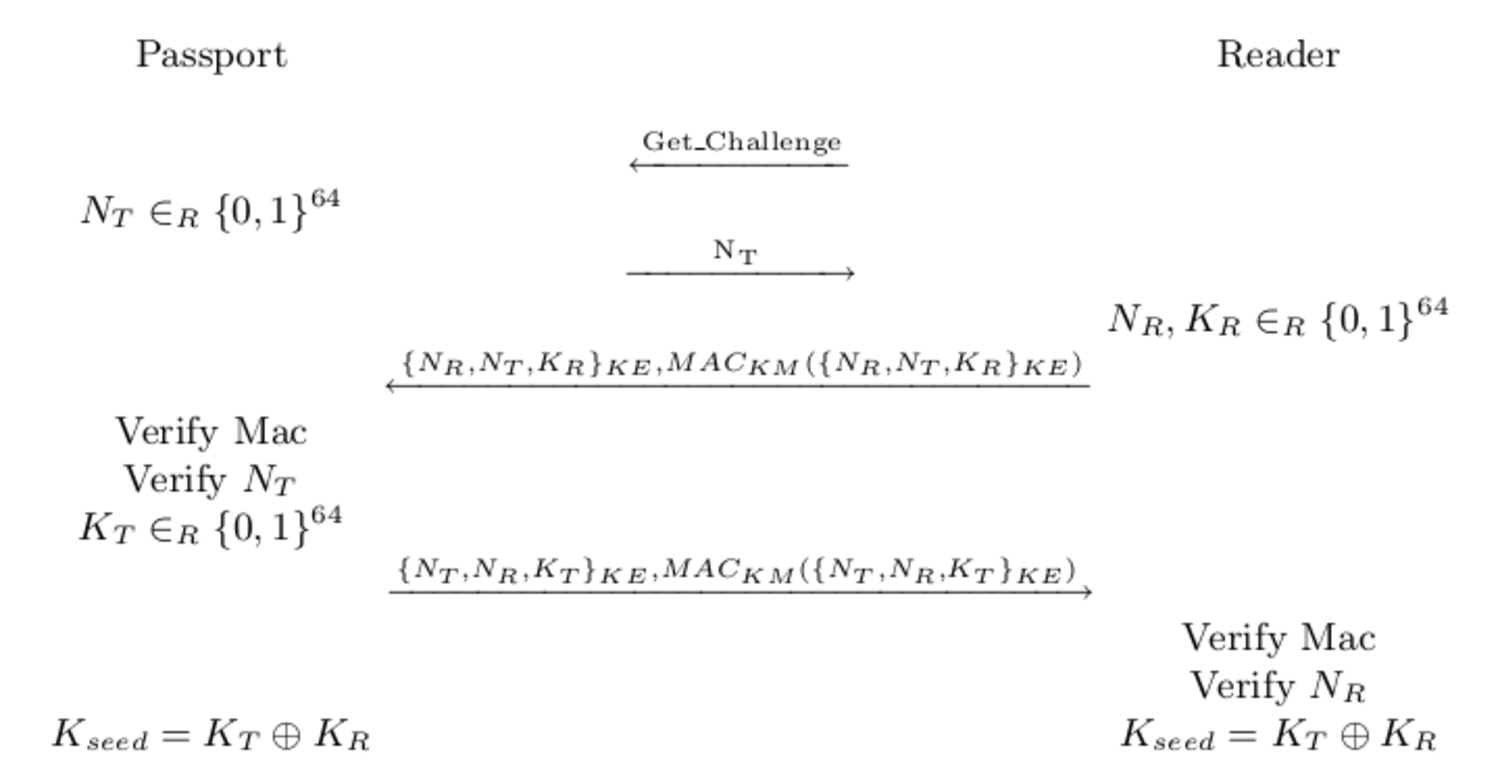
\includegraphics[scale=0.35]{BAC.pdf}
  \caption{BAC protocol sesion.}
  \label{fig:fig1}
\end{figure}

As we can see at the figure \ref{fig:fig1} once the tag receives the challenge from the reader, he answers 
by some encrypting information with the keys KE and KM where the reader has to be able to prove the 
knowledge of the keys from the MRZ. When the tag proves the authenticity, a session key KS-Seed 
is generated to encrypt all the communication.

\subsection{Ative Authentication}
As mentioned at \cite{JUAR2005}, in order to prevent cloning the \textit{AA} protocol was created. 
This protocol is more an anti-cloning feature because here the passport must prove 
to the reader that he has a private key as a response to a challenge previously received.

\subsection{Extended Access Control}
In \cite{NM12} is mentioned that in next generation e-passports EAC has being used 
instead of BAC because before proceeding with the same steps as BAC he verifies the 
authenticity of the reader by a certificate validation from the issuing passport’s country, 
certificate which must be transmitted in a safe way.

%\subsection{Citations}
%Citations to articles \cite{bowman:reasoning, clark:pct, braams:babel, herlihy:methodology},
%conference

\section{E-passports Attacks}
\label{sec:sec3}

\subsection{Cryptographic Weaknesses}
\label{subsec:crypt}
As we know, the \textit{Basic Access Control (BAC)} protocol establishes a secured channel between 
the \textit{RFID} tag and the reader in order to provide confidentiality and integrity to the 
data communication. \textit{BAC protocol} generates the encryption and authentication keys from the data 
present in passport's \textit {MRZ} (number, expiration, date of birth ) and it is demonstrable 
that the entropy of this data don’t reach at least the 80 bits suggested and can be worse 
with simple observations \cite{JUAR2005} \cite{02COPA}.\\
Liu, Kasper and others \cite{02COPA} had made a complexity analysis of the key space focused on 
demonstrate the low entropy of \textit{BAC keys} for two main passport’s nationality: Germany, 
Netherlands but easily extensible to other countries. The low entropy of key is caused 
first by the use of mainly numeric characters on passport number, 
second because of the stochastic dependency between passport number and its expiration 
date, and finally due to dependency of publicly available personal data. The analysis 
showed that in the best case, we know only public information and issuing state, the 
entropy reach \textbf {52.8 bits} for the German’s passports but it can fall to \textbf {20.4 bits} for 
Netherlands passports if we have a \textit{BAC keys database}. This low entropy is more disturbing 
when they estimated the time to find the \textit{MRZ} in 25h and less than 185ms 
respectively.

\subsection{Traceability}
\label{subsec:trace}

One of the most serious problem of e-passport is the possibility to trace them, that means that  
attackers are able to identify a passport that they knew before. According to Chothina and Smirnov 
\cite{CHTOM2010} this is possible because of the wireless lecture system of these 
\textit{MRTD (Machine Readable Travel Document)}.

The most interesting argument of these authors \cite{CHTOM2010} is that we can identify the passport using the 
security system that it uses to avoid unauthorized readers: \textit{BAC}. The attacker only need to record 
(eavesdropping) a session between the passport and an authorized reader (one that has access to MRZ), 
it can be done from a distance of 25m \cite{02COPA}, and when they come across another passport they send 
the \textit{\textbf{GET CHALLENGE} message} in order to get a nonce that the attacker will answer with the recorded message. 
As the \textit{ICAO standard} specifies that passports have to answer to all message using \textbf{ISO 7816} error codes, 
such as \textit{``6A80: Incorrect parameters''} or \textit{``6300: No information given''}, them the answer of passport to 
recorded message will be useful to identify him because they send a specific message when \textit{MAC check} 
fails or rises  (french passports) or maybe because the answer time is greater when \textit{MAC check} succeed. 
In both cases, if \textit{MAC check} is correct we are addressing to the same passport.

All this attacks have been made without any victim’s passport contact, and the closest communication 
(BAC challenge) is possible a 50cm away \cite{CHTOM2010}.

\subsection{Physical-layer Weaknesses}
\label{subsec:phy}
All the information that we can extrait from e-passport is a potential threat for the owner or for 
the national security of the country (expediter or receptionist) but this information is not necessary 
linked to cryptographic process in \textit{MRTD}, sometimes it is more accessible than we think. This is the 
case of the attacks to communications protocols in physical layer, maybe useful with all \textit{RFID tags} 
but when they are linked to e-passports they can give us additional information.

First we can talk about Danev, Heydt-Benjalin and Capkun \cite{05DABO2009} work, they have tested their method 
to identify the manufacturer of RFID smart cards with an equal error rate of 2.43\%. This error rate 
makes the RFID transponders identification possible in practical situations including e-passports. 
The attacker only need a recorded signal and then the statistic analysis of spectral features. 
There are not a lot of RFID manufacturers and, of course, nations have to buy the RFID tag of their 
e-passports to some of them. If we can determine the manufacturer of the smart card in the passport 
then we will be closer to identify its nationality. This information will be useful to determine the 
MRZ as we have seen before \ref{subsec:trace}.

In the other hand, in logical level the communication reader-passport use \textit{Applications Protocol 
Data Units (APDUs)} which are specified in \textit{ISO 7816} standard. Of course this standard have some status 
words defined like \textit{“No error (9000)”, “Unknown(6F00)”} and more but the \textit{ICAO} guidelines for 
e-passports are not specific about the logical response to every command, that is the reason why 
all nations have the freedom to use the \textit{APDUs} as they want. This liberty to chose the response of 
logical commands makes possible to Richter, Mostowski and Poll \cite{03HENN} identify the nationality of 
passport using a set of 7 commands and watching the answer of every passport to them. Ten passports's 
nationlities have been identified by using this little command set; in order to increase the number of 
known nationalities would be necessary to use some others commands which is still possible.


\subsection{Cloning}
As mentioned in \cite{MHTR07}, once the reader and the tag have passed BAC, AA is implemented. 
As it was already mentioned the objective of this protocol is to the prevent cloning, 
so once the reader sends the challenge to the tag it responds immediately responds with a 
WAIT message leaving a gap of five seconds which finally are about four seconds because the 
tag takes approximately one second to perform the private key validation. 
So a possible scenario (as dictated at \cite{MHTR07}) is when somebody for 
example at an hotel forgets his passport at the reception, somebody at the reception 
could have access to the MRZ sends those values to somebody at the border and with a 
device registers that, passes the BAC and once at AA he replays all messages from the 
reader to and from the true passport all of that in even in less than four seconds.

\section{Conclusions}
\label{sec:sec4}
Our revision shows that e-passports have some weaknesses that could make some information accessible. This is an international identification document and all its data compromise the holder and the countries involved. Due to its importance, all efforts to increase the confidentiality of this information is well seen. We present below our conclusions and some recommendations.

First, we have seen that most vulnerabilities are due to \emph{ICAO} standard for this technology. This guide is not so specific and give a lot of liberty hence every country implements almost his own version. The \emph{ICAO} have to specify all the interactions (even error messages and response time)  between the passport and the reader for every level of communications (application, logical, physical). Without this regulations, the fragilities of subsections \ref{subsec:trace} and \ref{subsec:phy} will be always there.

Secondly, we clap the use of \emph{BAC protocol} in order to secure the channel. But will be necessary to change the key derived from \emph{MRZ}. The use of \emph{MRZ} give some additional security to authentify the reader, but the actual information inside has not enough entropy [Subsection \ref{subsec:crypt}] to assure a secure key. Add random alphanumeric information could help.

Finally, the countries must reconsider the use of RFID tag in passports. Until now wireless communication is really the main vulnerability of e-passports. For holders, it is impossible to know when they are transmitting and it can be caused by a distant reader. For countries it is difficult to limit the wave scope and, as we saw, guarantee its confidentiality. A smart card with mandatory contact can be near the transfer rate of RFID and can make the same function.

The invulnerability is the defiance for the next generation of e-passport. Important changes must come because the safety of millions is involved. 

\bibliographystyle{abbrv}
\bibliography{sigproc}  % sigproc.bib is the name of the Bibliography in this case
% You must have a proper ".bib" file
%  and remember to run:
% latex bibtex latex latex
% to resolve all references
%
% ACM needs 'a single self-contained file'!
%

\balancecolumns
% That's all folks!
\end{document}
